%________________________________________
%CaRS Move I "Establish a territory" (Situation):
% * Important area
% * Introducing and reviewing items of previous  research <--(ToDO)
Ship dynamics predictive models have a wide range of applications, e.g., safety enhancements, route planning and optimization, autonomous shipping, etc., \citep{aslam_internet_2020}.
Ship manoeuvring is a sub field of ship dynamics with well established system based models such as: \citet{abkowitz_ship_1964,nomoto_steering_1957,norrbin_theory_1971}, and the MMG model \citep{yasukawa_introduction_2015}.

Captive model test is the classical method to identify the parameters within these models. However, for the full scale ships, this method is not practically applicable, while computational fluid dynamics (CFD) with either direct simulations or virtual captive tests (VCT) has emerged as an interesting option \citep{liu_predictions_2018,li_ship_2022}.
The CFD requires a complete understanding of the system. Acquiring such knowledge may be possible for some simplified scenarios, but large modelling uncertainties from wind, wave and current are expected when applied in a complex sea environment \citep{miller_ship_2021}. 
Even if the sea is flawlessly modelled, long-term predictions with high accuracy will be exposed to deterministic chaos \citep{lorenz_deterministic_1963}.
Together with the other drawbacks of CFD in manoeuvring -- such as high computational costs -- data driven models have become an attractive alternative or complement, with an increased number of publications in the past 10-15 years %(shown in Fig.\ref{fig:pub_overview})
-- especially within the field of autonomous ships \citep{ahmed_survey_2023} where it is important to predict the ships’ trajectories to avoid collision. 

The keywords and their connections of most recent research activities related to ship maneuvering modelling are presented in \autoref{fig:pub_overview}, where the size of the circles indicates how often those keywords occurred in those research articles. All the papers state that their proposed regression-based methods can effectively estimate the hydrodynamic coefficients of a ship’s maneuvering system. However, most of those regression methods are based on that the exact “physical” model is assumed known, i.e., the regression is based on “simulation” data. This is clearly indicated in \autoref{fig:pub_overview} that both keywords of “simulation” and “maneuvering simulation” are directly connected with others, while their sizes are also large.
Most of the simulations (as in the keywords) were based on the model in \citet{fossen_handbook_2021}, such as the Gaussian process regression method in \citet{xue_system_2020}, and support vector machine method in \citet{wang_identification_2019}, \citet{wang_parameter_2021}, etc. Recently, the support vector machine and neural network methods were also used to identify the parameters of ship dynamic models using data from some benchmark model tests with well-known ship maneuverability (Simman, SHOPERA, etc.), as in e.g., \citet{wang_kernel-based_2020}, \citet{wakita_neural_2021}. The identified maneuvering models were validated by comparing their capabilities for trajectory prediction with either simulated or well-controlled model test results. However, the accuracy of those identified models to describe the ship’s physical dynamic performance, e.g., various forces acting on ships, is rarely mentioned. But such dynamic performance is essential to determine the feasibility of the identified model for the application of a ship’s operation in real sea environments, i.e., with drifting caused by wind and current.
%%
\begin{figure}[h]
  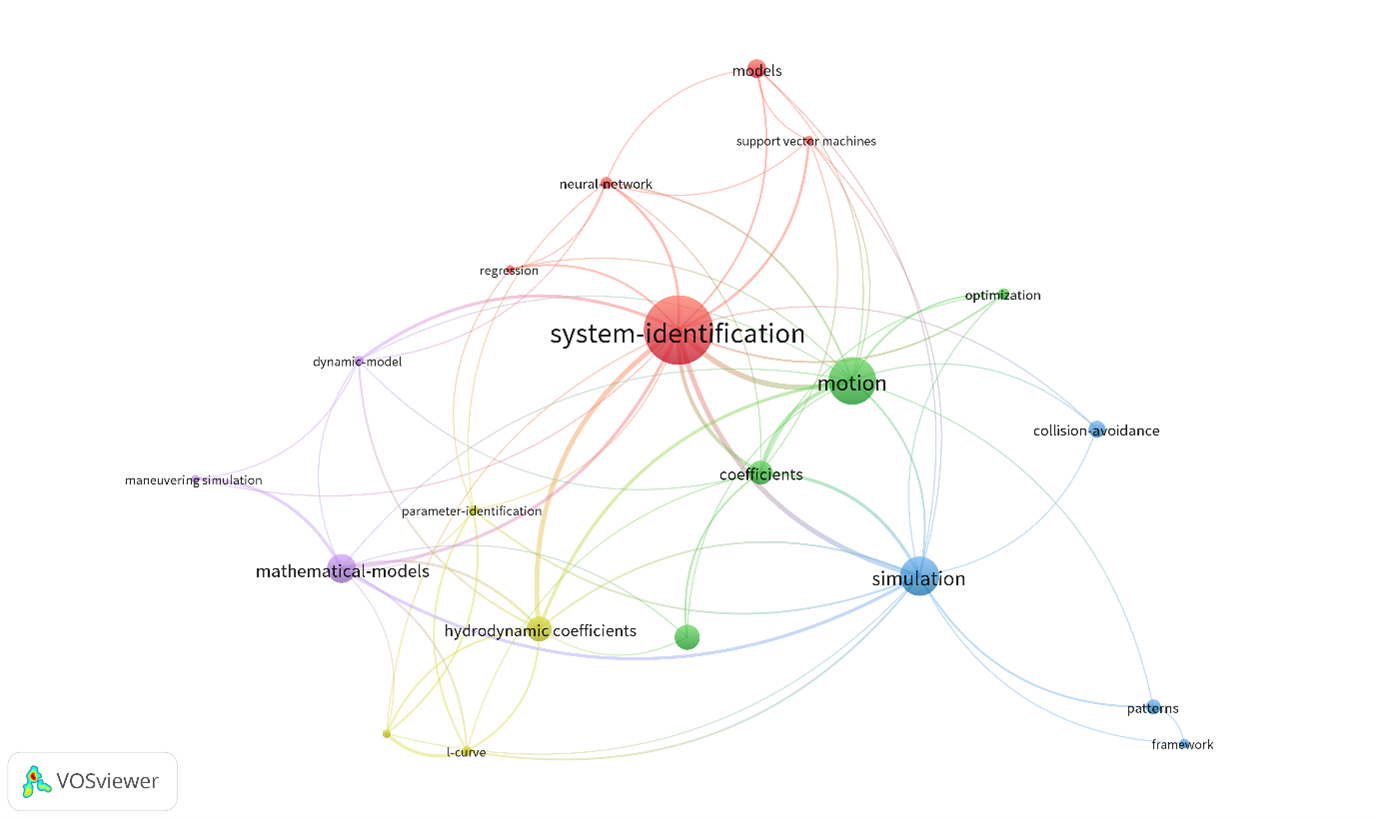
\includegraphics[width=\textwidth]{figures/keywords.png}
  \caption{Research topics within the field of ship maneuverability system identification.}
  \label{fig:pub_overview}
\end{figure}
%%
%fication_1976} to develop a linear manoeuvring model that utilized manually recorded data in 1969 aboard the Atlantic Song freighter with Kalman filter (KF) and maximum likelihood estimation. 
%a_system_2015}, a 3 degree of freedom model by \citet{shi_identification_2009}, and a recursive EKF by \citet{alexandersson_system_2022}.
%KF for handling nonlinear systems, was used in \citet{revestido_herrero_two-step_2012}.
%\citet{zhu_parameter_2017}, and \citet{wang_parameter_2021}. 

%
%________________________________________
%CaRS Move II "Establish a niche" (Problem):
% * counter claim?
% * gap?
% * question       <------
% * continuation?
The regressors of the data-driven ship manoeuvring models are often strongly linearly dependent. This multicollinearity is a well known issue in parameter identification, that may lead to parameter drift and poor generalization. The parameters are thus mathematically correct but physically incorrect \citep{luo_parameter_2016}. 
An example of generalization is when a model identified on calm water data is exposed to wind, where a drift angle is now needed to maintain a straight course. This wind state is rare in calm water manoeuvring tests, where the drift angle is almost exclusively accompanied by yaw rate (see \autoref{fig:phase_portrait}); 
The regression will thus have problems to distinguish between these quantities.
% Wengang fixes a better figure here...
%This drifting (side forces) is rarely investigated as shown in %\autoref{fig:pub_overview}.
%
\begin{figure}[h]
  \centering
  \includesvg{figures/multicollineraity.multicollinearity.svg}
  \caption{Phase portrait where the combination of drift angle and yaw rate is shown for zigzag10/10, and zigzag20/20 wPCC model tests.}
  \label{fig:phase_portrait}
\end{figure}
Using more informative data or simplifying the model -- when possible -- and thereby reducing the number of parameters, is one of the most researched ways to mitigate the multicollinearity. Other possible remedies are the difference method \citep{luo_parameter_2016}, principal component analysis (PCA), and partial least squares regression \citep{jian-chuan_parametric_2015}. 
%________________________________________
%CaRS Move III "Occupy the niche" (Solution/Evaluation):
% * outline purpose?                        <--
% * list research questions?                <--
% * announce principal findings?            
% * stating the value of present research?
% * article structure?                      <--

More remedies are however needed; Therefore, in this paper, a physics informed manoeuvring model (PI model), which features a new semi-empirical rudder model based on semi-empirical formulas from the literature, is proposed.

The objective of this paper is to investigate if the PI model is physically more correct than a physics uninformed model (PU model), when they are both identified from zigzag model tests, and also to investigate how this affects the generalization.
To evaluate the physical correctness, a wind-powered pure car carrier (wPCC) test case is studied. 
This ship has much larger rudders than conventional ships -- to improve the sailing performance -- 
which increases the demand for a physically correct rudder modelling.

A brief description of the workflow of this research is shown in \autoref{fig:methodology}.
The PI and PU models are identified on free sailing model tests via inverse dynamics \citep{faber_inverse_2018} and regression (ID regression). To assess the physical correctness, a reference model is established, where the PI model is instead identified on a VCT dataset. This reference model -- which is based on CFD -- is assumed to be a sufficiently correct representation of the real ship model physics.
Verification and comparisons between the models are carried out on the free sailing model tests. The generalization of the models are then studied on an idealized wind condition.
%
\begin{figure}[h]
  \centering
  %\includesvg[width=\columnwidth, pretex=\scriptsize, height=12cm]{figures/methodology2.svg}
  \includesvg[pretex=\centering\fontsize{7.5}{8}]{figures/methodology2.svg}
  \caption{Research workflow.}
  \label{fig:methodology}
\end{figure}

The left of the paper is organized as follows; The proposed PI model is first presented together with the PU 
 model in \autoref{sec:ship_models}, while some mathematical details of the models are given in the appendix. 
The developed methodology framework to identify parameters within the PI model is described in \autoref{sec:methodology} -- including the VCT regression, and the inverse dynamics. The case study ship is briefly described in \autoref{sec:case_study}, as well as some known parameters of the ship's manoeuvring model. Results are presented in \autoref{sec:results}, followed by some key conclusions of this research in \autoref{sec:conclusions}.